\insertmeeting 
	{Prototyping Party} 
	{09-28-22} 
	{Hagerty High School}
	{Jorge, Nathan, Ritam, Robert, Samantha}
	{Images/RobotPics/robot.jpg}
	{1:30 - 3:30}
	
\hhscommittee{CAD}
\noindent\hfil\rule{\textwidth}{.4pt}\hfil
\subsubsection*{Goals}
\begin{itemize}
    \item Create Ackerman skeleton
    \item Design prototype for front wheels of drivetrain


\end{itemize} 

\noindent\hfil\rule{\textwidth}{.4pt}\hfil

\subsubsection*{Accomplishments}
Getting right into CAD, we started this meeting by creating a skeleton, or a basis for how the design would be laid out upon which we can base the dimensions for the entire design. One of the most important features of the skeleton is representing the Ackermann steering ratios which we learned about in the last hardware meeting. Creating a sketch we made construction lines representing the wheels, chassis, ackermann linkage, and turning path (figure 1). All of this will help us find the correct measurements for the steering arms and will allow us to easily change the dimension of the whole design without breaking it or having to redesign.

Using the information for the skeleton, we started creating a steering knuckle, a part that attaches the wheel to the rest of the chassis, allowing the wheel to swivel (figure 2). The next part we created is a basic chassis structure. Because this is just a prototype, we didn’t design the full body of the robot, instead creating just the front section, enough to hold the steering knuckles together (figure 3). We also added a point where a carbon fiber tube can connect to the front of the chassis in case we want to expand the prototype later to include back wheels. The last part we made was the tie bar of the ackermann linkage which allows both of the turning knuckles to turn at different angles, following the circular paths of different radii caused by having 2 steering front wheels (figure 4). We decided to link all of the joints together with simple nuts and bolts, because although they aren't the most efficient and long lasting way to create a rotating joint, it is the easiest and they will be sufficient for a prototype. We put everything together in an assembly, making sure it all fits and works together as intended. With the design done, we 3D printed the parts, excited to see how they will turn out.

 

\begin{figure}[ht]
\centering
\begin{minipage}[b]{.48\textwidth}
  \centering
  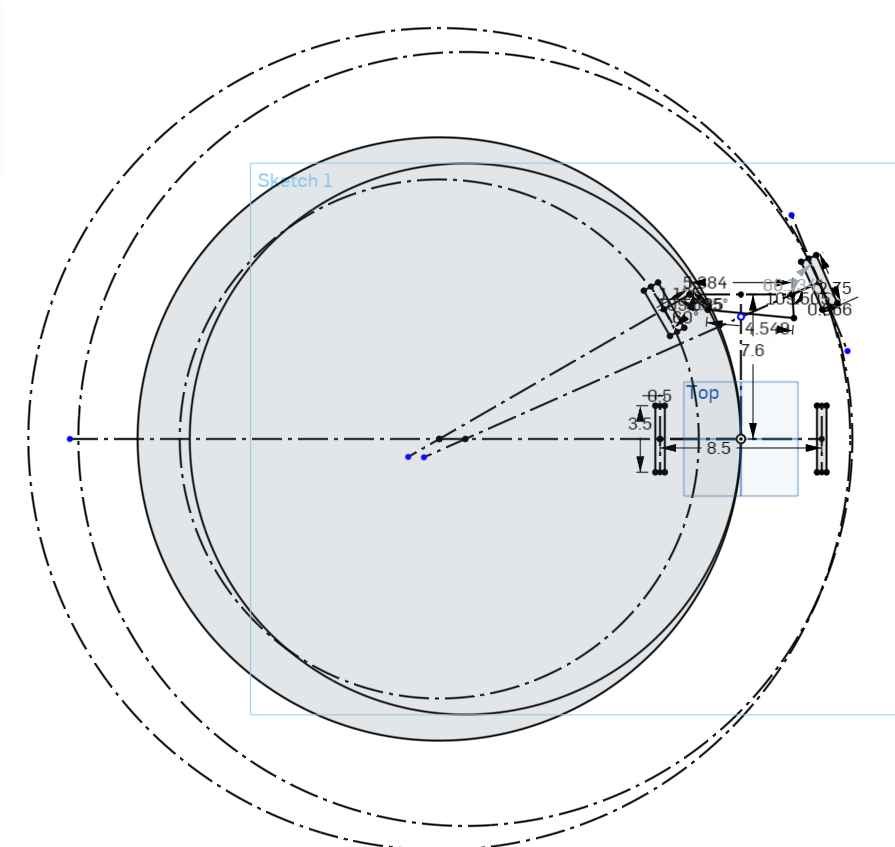
\includegraphics[width=0.95\textwidth]{Meetings/September/09-28-22/9-28-22_CAD_Figure1.PNG}
  \caption{Drive team on field}
  \label{fig:pic1}
\end{minipage}%
\hfill%
\begin{minipage}[b]{.48\textwidth}
  \centering
  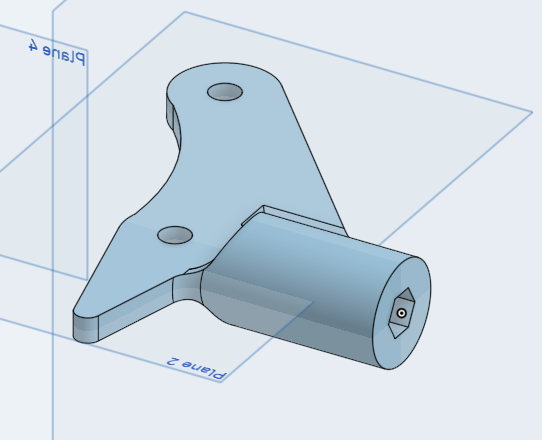
\includegraphics[width=0.95\textwidth]{Meetings/September/09-28-22/9-28-22_CAD_Figure2.PNG}
  \label{fig:pic2}
\end{minipage}
\end{figure}

\begin{figure}[ht]
\begin{minipage}[b]{.48\textwidth}
  \centering
  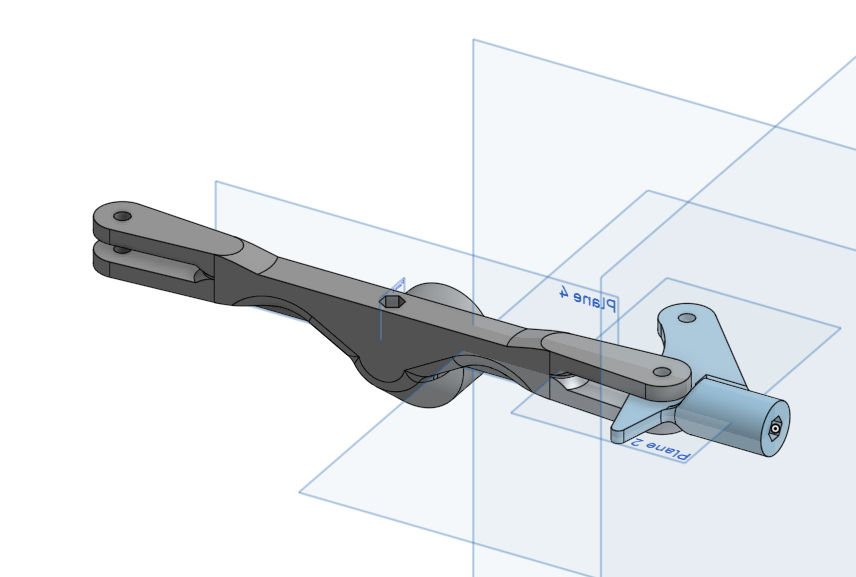
\includegraphics[width=0.95\textwidth]{Meetings/September/09-28-22/9-28-22_CAD_Figure3.PNG}
  \label{fig:pic2}
\end{minipage}

\begin{minipage}[b]{.48\textwidth}
  \centering
  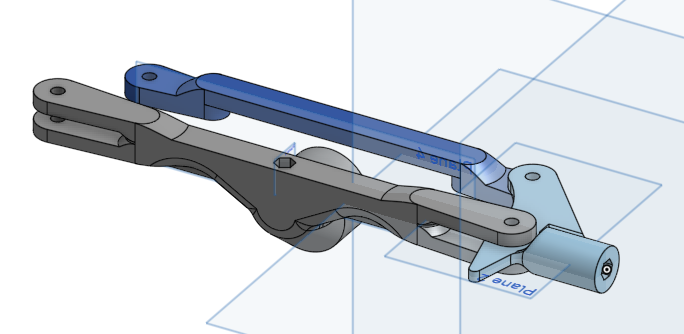
\includegraphics[width=0.95\textwidth]{Meetings/September/09-28-22/9-28-22_CAD_Figure4.PNG}
  \label{fig:pic2}
\end{minipage}
\end{figure}

\whatsnext{
\begin{itemize}
    \item Assemble Ackerman steering prototype
    \item Make sure the prototype works properly

    
\end{itemize} 
}
